\def\year{2015}
\documentclass[letterpaper]{article}
\usepackage{aaai}
\usepackage{graphicx}
\usepackage{algorithm}
\usepackage[noend]{algpseudocode}
\usepackage{amsmath}
\usepackage{amssymb}
\usepackage{amsthm}
\usepackage{etoolbox}
\usepackage{color}
\usepackage{changepage}
\usepackage{csquotes}
\usepackage{tabularx,booktabs,multirow}
\usepackage{longtable}
\usepackage{framed}

\pdfinfo{
/Title (Learning Constraints and Optimization Criteria)
/Author (Samuel Kolb)}
\setcounter{secnumdepth}{0}  

\graphicspath{{Graphics/}}

\newcommand{\sym}[1]{\ensuremath{\mathcal{#1}}}
\newcommand{\svm}{SVM$^{rank}$}

\newtheorem{definition}{Definition}[section]
\newtheorem{question}{Question}
\AfterEndEnvironment{definition}{\noindent\ignorespaces}

\theoremstyle{definition}
\newtheorem{example}{Example}
\newtheorem{experiment}{Experiment}[question]
\newtheorem{observation}{Observation}[question]

\setlength{\tabcolsep}{6pt}

\begin{document}

\title{Learning Constraints and Optimization Criteria}
\author{
  Samuel Kolb\\
  KU Leuven, Leuven, Belgium\\
  samuel.kolb@cs.kuleuven.be
}

\maketitle

\begin{abstract}
This paper presents a system that is able to automatically learn both constraints from examples and optimization criteria from rankings.
Both hard and soft constraints can be learned and constraints are represented as first order logical clauses.
Choosing such clauses as representations enables the use of ILP techniques such as clausal discovery.
In this research, optimization criteria are represented as weighted clauses.
For all examples, the clause learning system could find the essential constraints efficiently.
The learning system for optimization criteria is shown to achieve accurate results and can learn criteria that identify the correct optimal solution even for few examples and noisy rankings.
Finally, a procedure is outlined that allows weighted first order logic clauses to be used for optimization in practice.
\end{abstract}

% -------------------------------------------------
% Introduction
% -------------------------------------------------

\section{Introduction}
This paper introduces an approach for learning constraints and optimization criteria.
Using constraints and optimization criteria such as the ones proposed in this paper allows problems to be modeled \emph{declaratively}.
This means that the representation is decoupled from the process of finding a (optimal) solution for the problem.
However, non-experts often experience difficulties when modeling a problem using constraints \cite{Wallace:PrinciplesCP}.
The first goal of this research is to automate the step of modeling a problem, in order to, amongst others, make constraint solving more accessible.
In this approach a few examples of what a user considers valid solutions are used by a computer system to find constraints.
These constraints can then be used by an existing constraint solver.

Constraint learning attempts to find constraints automatically given examples.
By using first-order logical clauses as representation for constraints, techniques from Inductive Logic Programming (ILP) can be used for learning.
Hereby, this research follows the same approach as \cite{Lallouet:LearningCP}, exploiting parallels between ILP and constraint learning.
In this case, the clausal discovery algorithm \cite{DeRaedt:ClausalDiscovery} is used to find constraints.

There has been increasing interest in formulating declarative models for constraint satisfaction as well as optimization problems.
By identifying soft constraints that are only satisfied by some examples and assigning weights to them based on their importance, an optimal solution can be sought.
The use of weighted soft constraints to model user preferences is inspired, amongst others, by the research of \cite{campigotto2011active}.
Their work examines attempts to obtain similar results in an interactive context for propositional constraints.
In this research, first-order constraints are used and optimization criteria are modeled using a first-order version of weighted MAX-SAT.
This paper also outlines how these constraints can be used in an existing solver to obtain an optimal solution in practice.

Since the underlying goal of this research is to facilitate the generation of a formal representation, the input format aims to be easy to use.
It has been a key focus to make reasonable assumptions concerning the knowledge a user can provide.
One important difference compared to similar research (including \cite{campigotto2011active}) is that users provide partial rankings over examples instead of absolute scores.

This paper is based on research that has been conducted during the course of my masters thesis~\cite{kolb2015thesis}.
The key contribution presented in this paper is a novel approach for learning weighted first order clauses from rankings to capture user preferences.
In this context an implementation of clausal discovery has been realized that supports soft constraints.
Moreover, an approach to obtaining optimal solutions for the weighted first order clauses is presented.

% -------------------------------------------------
% Background
% -------------------------------------------------

\section{Background}
In this section a brief overview of the important concepts and relevant literature will be provided.

\paragraph{Clauses}
First-order logical clauses consist of a disjunction of literals.
Literals are defined as being either an atom (positive literal) or a negated atom (negative literal).
Clauses are often expressed using a body and a head: $\mathit{head} \leftarrow \mathit{body}$.
Hereby, positive literals are grouped in the head and negative literals are grouped in the body.
%For example, $\lnot a_1 \lor \lnot a_2 \lor a_3 \lor a_4$ corresponds to the clause $a_3, a_4 \leftarrow a_1, a_2$.

Terms are used to reason about objects and consist of either constants denoting specific objects or variables that can represent any object.
In this paper constants will be written in uppercase ($\mathit{John}$) and variables in lowercase ($\mathit{x}$).
Relations between logical objects are represented by predicates, consisting of a predicate symbol and a set of terms (e.g. $\mathit{married(John, x)}$).
Predicates are atoms and can be assigned a truth value.

\paragraph{Learning constraints}
Constraint learning is a hard problem.
The search space of constraints is typically very large and, unlike in typical machine learning problems, there are usually only few examples to learn from.

Different systems attempt to learn constraints using different methods.
The problem of having little examples can be alleviated by interactively generating data.
Both the systems Conacq2 \cite{bessiere2007query} en QuAcq \cite{bessiere2013constraint} generate (partial) examples and query the user about their validity.

ModelSeeker \cite{Beldiceanu:ModelSeeker} attempts to structure the problem variables in different ways.
The system then tests for different global constraints whether they hold within this structure.
This approach allows for constraint learning from a few examples.

As mentioned earlier, the research of \cite{Lallouet:LearningCP} already tried to use ILP techniques to learn constraints.
In their approach, the search space of constraints is explored in a bidirectional manner, primarily using negative examples.

\paragraph{Clausal Discovery}
The clausal discovery algorithm proposed by \cite{DeRaedt:ClausalDiscovery} attempts to learn first order logic clauses from positive examples.
Using a refinement operator, the search space is traversed by incrementally generalizing clauses until they cover all examples, starting from the empty clause~($\square$).
The result set consists of the most specific clauses covering all examples.

\paragraph{Logic Solver}
The logic system IDP \cite{de2013prototype,wittocx2008idp} is used to calculate whether examples satisfy clauses and is used as a theorem prover.
It supports an extension of first order logic ($FO(\cdot)$) and can also be used to generate new solutions.
Background knowledge is given as an IDP theory.

\paragraph{Optimization}
The Boolean Satisfiability Problem (SAT) attempts to determine whether a propositional formula can be satisfied.
Formulas can be rewritten into a special form called the conjunctive normal form (CNF), which consists of a conjunction of clauses (disjunctions).
An extension of this problem is the Maximum Satisfiability Problem (MAX-SAT).
In MAX-SAT the amount of satisfied clauses is maximized.
By assigning positive integer weights to clauses and maximizing the sum of the weights of satisfied clauses, one obtains the weighted MAX-SAT problem.
The work by \cite{campigotto2011active} attempts to learn propositional formulas and weights automatically using examples and absolute scores.
Inspired by their results, this research tries to learn first-order logic clauses and weights using examples and rankings.
The resulting optimization problem can be seen as an extension of weighted MAX-SAT in which the clauses are in first-order logic.

% -------------------------------------------------
% Problem Statement
% -------------------------------------------------

\section{Problem Statement}
The research presented in this paper aims to learn constraints and optimization criteria based on positive examples and user preferences.
Since it aims to simplify the process of generating formal representations it should be easy to use and require input that a user can reasonably be expected to provide.

\subsection{Constraint learning}
\emph{Given a set of examples and a limit $t$, the goal is to find maximally specific clauses that are satisfied by at least $t$ of the given examples.}
\\\\
Examples consist of a domain and an exhaustive description of all relations that hold on the domain objects.
The learned clauses are domain-independent and contain only variables.

% \begin{example} " TODO - necessary?"
%   Consider sudoku as an example of a problem where hard constraints are to be found.
%   Given one or more solved sudokus, the learning system has to identify the rules of the game.
%   Since the learned clauses only contain universally quantified variables, for example $4 \times 4$ sudokus could be used to find constraints.
%   The learned constraints are independent of the size of the sudoku and can also be used to solve $9 \times 9$ sudokus, for example.

%   In some problems, one is interested in regularities that  often but not always occur.
%   An example would be regularities in certain types of buildings.
%   While certain regularities would occur in many buildings, there are often exceptions and different styles.
%   In this case, one could attempt to find constraints on the structure of the floor plans that are satisfied by a given amount of examples.
% \end{example}

\subsection{Learning optimization criteria}
\emph{Given a set of examples and a set of partial rankings over these examples, the goal is to identify soft constraints and weights learn such that the order described by these optimization criteria maximally corresponds with the given rankings.}
\\\\
The soft constraints consist of clauses that are satisfied by some but not all of the examples.
They can be identified using a system that implements the constraint learning task.
Partial rankings reason over sets of examples and describe an order over them (e.g. the ranking $e_i > e_j$ expresses the users preference of example $e_i$ over example $e_j$).
The weighted clauses (i.e. tuples $(weight, clause)$) can be used to calculate a score for every example:
\begin{eqnarray*}
  score(e) = \sum\limits_{(\mathit{w}, \mathit{c})} \mathit{w} \cdot \mathbf{1}_{c \text{ covers } e}
\end{eqnarray*}

\begin{example}[Moving]
  \label{ex:moving}
  Consider the scenario moving to a new city.
  The user has to choose a job, a place to live and a school.
  There are multiple job offers, houses and schools available across different areas of the city.
  User provided examples include a choice of where to work, where to live and what school is chosen.
  By comparing and ranking some of the examples, the user can express his preferences.
  Weighted soft-constraints can now be learned and used to identify the best choice.
  In this case, a possible soft constraint could be that the school and work place are in the same area.
  The weights that have been learned indicate how desirable or how undesirable a constraint is.
  Since the constraints are domain independent they can be used for any (unseen) city.
\end{example}

Aside from learning optimization criteria, this paper presents an approach to use these optimization criteria to find an optimal solution in practice.

% -------------------------------------------------
% Approach
% -------------------------------------------------

\section{Approach}
In this research, both constraint learning and learning optimization criteria were implemented.
Clauses are learned using examples.
The clause learning implementation uses the IDP system to test if clauses satisfy the examples and identify redundant clauses.
When learning weighted clauses, soft constraints are first identified in the examples using the clause learning implementation.
These constraints are assigned weights based on the given rankings.

\subsection{Input}
The input consists of global definitions and a set of examples.
Definitions consist of either typing information or predicate definitions.
Typing information relates directly to the problem domain, improves the accuracy and efficiency of the learned clauses and is usually easy to provide for the user.
Predicate definitions define predicate symbols and the types of their terms.
Two special types of predicates are allowed: calculated predicates and symmetric predicates.
Calculated predicates are not included in examples, instead background knowledge is used to generate them.
This background knowledge is passed directly to the IDP system.
Symmetric predicates are predicates for which the order of the terms does not matter.
Every example contains a domain consisting of a set of constants and an exhaustive list of the relations (predicates) that hold on these constants.
If optimization criteria are to be learned, a set of pairwise over the given examples is also provided.
Rankings are used instead of absolute scores since rankings only concern few examples at a time.
Because rankings only ask for relative positioning of a few examples, they are easier to provide.

\begin{example}
  \label{ex:moving-input}
  Consider the moving problem (example~\ref{ex:moving-input}).
  A model could, for example, use a type \textit{Area} and predicate definitions low\_crime(\textit{Area}), cheap(\textit{Area}), school\_in(\textit{Area}), work\_in(\textit{Area}) and live\_in(\textit{Area}).
  Examples would that specify various areas $A_i$ and describe the conditions (e.g. cheap($A_1$), low\_crime($A_2$)) as well as the users choices (e.g. school\_in($A_2$), work\_in($A_2$), live\_in($A_1$)).
  % Imagine a problem that describes humans with a type \textit{human} and predicates human(\textit{human}), male(\textit{human}) and female(\textit{human}).
  % An example could contain the constants S and A, both of type \textit{human}, and the relations: human(S), human(A), male(S), female(A).
  % Clauses to be learned would be: human(x) $\leftarrow$ male(x), human(x) $\leftarrow$ female(x),  female(x) $\lor$ male(x) $\leftarrow$ human(x) and \textit{false} $\leftarrow$ female(x) $\land$ male(x).
\end{example}

\begin{algorithm}
  \caption{The clausal discovery algorithm}
  \label{alg:cd}

  \begin{algorithmic}
  \State $Q \gets \{\square\}$, $\sym{T} \gets \{\}$
  \While{$\lnot isempty(Q)$}
    \State $c \gets next(Q)$
    \If{$covers(c, \textit{Examples})$}
      \If{$\lnot entails(\sym{T}, c)$}
        \State $\sym{T} = \sym{T} \cup c$
      \EndIf
    \Else
      \State $Q \gets Q \cup \rho(c)$
    \EndIf
  \EndWhile
  \State $\sym{T} \gets prune(\sym{T})$
  \State \Return \sym{T}
  \end{algorithmic}
\end{algorithm}

\subsection{Clausal Discovery}
The clause learning system is based on the clausal discovery algorithm (alg.~\ref{alg:cd}).
The logical system IDP is used for two essential functions: $\mathit{covers}$ and $\mathit{entails}$.
The $\mathit{covers}$ function calculates which examples are covered by a clause.
The $\mathit{entails}$ function calculates whether an accepted clause is logically entailed by background knowledge or clauses that are already in the result set.

Starting with the empty clause, clauses are refined until they cover enough examples.
If a clause covers enough examples it is added to result set, provided it is not entailed by background knowledge or other clauses in the result set.
To avoid extensive calls to $\mathit{covers}$ and $\mathit{entails}$, two additional tests are used.
The subset-test rejects clauses that are supersets of a clause that covers the same or all examples and has been accepted earlier.
Because clauses can be formulated in multiple ways, a representative-test is used to remove clauses that are not in canonical form.

In the refinement step, clauses are extended to be more general and potentially cover more examples.
The refinement operator uses a list of atoms that may be added to a clause.
This list is calculated in advance, given a maximal amount of variables.
Within the body and head of a clause, atoms may only be added in a specific order to avoid generating redundant clauses.
Object Identity is used to specify that variables with different names must denote different objects.
Additionally there are two syntactic restrictions.
Clauses must be connected (i.e. new atoms must always contain a variable that has already occurred) and range-restricted (i.e. no new variables may be introduced in the head of the clause).

\subsection{Optimization}
The first step in finding weighted soft constraints is to identify soft constraints by using the constraint learning system with a (low) threshold.
Examples are characterized by the soft constraints (clauses) which they satisfy.
Therefore, every example~$e$ can be translated to a vector of boolean features by introducing a feature~$f_i$ for every clause~$c_i$, with $f_i = \mathbf{1}_{c_i \text{ covers } e}$.
Existing software can be used to learn a linear scoring function $\sum_i w_i \cdot f_i$ over these features based on the given rankings.
For an unseen example, the feature vector is computed by calculating what clauses cover the new example.
The scoring function can then be used to calculate a score for that example.

\begin{example}
  Consider examples~$e_1, e_2, e_3$, rankings $e_1 > e_2, e_2 > e_3$ and clauses $c_1, c_2, c_3$.
  If the clauses cover examples according to table~\ref{tbl:cover_examples}, then, for example, the function $(1 \cdot c_1) + (0\cdot c_2) + (-2\cdot c_3)$ perfectly models the given rankings.
  A new example that is covered by~$c_1$ and~$c_2$, would be assigned a score of $1$, according to this function.
  This score has no value in the absolute sense, it can only be used to compare it to other examples ranked by the same function.
  In this example clause~$c_1$ represents a desirable property, clause~$c_2$ is ignored because it does not influence the ranking and clause~$c_3$ represents an undesirable property.

  \begin{table}
  \caption{Clause coverage}
  \label{tbl:cover_examples}
  \begin{tabularx}{\linewidth}{c|l|X}
    \textbf{Example} & \textbf{Covered by} & \textbf{Feature vector}\\
    \toprule
    $e_1$             & $c_1$               & (1, 0, 0) \\
    $e_2$             & $c_2$               & (0, 1, 0) \\
    $e_3$             & $c_1$, $c_2$, $c_3$ & (1, 1, 1) \\
  \end{tabularx}
  \end{table}
\end{example}

The \svm{} software was chosen to find the scoring function since it uses a linear model and offers an efficient implementation.
The weights that it assigns to the features can be used directly as weights for the optimization criteria.
The input format that is used by \svm{} is also supported by many other learn-to-rank implementations.
Therefore, other linear ranking systems such as Coordinate Ascent \cite{metzler2007linear} could also be used.

\subsection{Optimal Solution}
Solvers, such as IDP, can use clauses directly as hard constraints to generate a solution.
There is no solver that can use the chosen optimization criteria directly.
Weighted MAX-SAT solvers use propositional clauses and only allow for positive weights.

This optimization task can be solved in IDP, using inductive definitions, aggregates and minimization.
The only limitation is that the current version only supports integer values.
Therefore, the weights of the clauses are divided by the smallest absolute weight, multiplied by a constant and rounded to the closest integer if necessary.

In order to model the optimization problem in IDP, every clause $c_i$ with variables $v_1, ..., v_n$ is represented by a number $i$. For every clause a predicate $t(i)$ is added to capture the truth value of the clause.
A function $\mathit{cost}(i)$ specifies the cost of not satisfying the clause, which is equal to the weight of the clause.
\begin{eqnarray*}
  t(i) \Leftrightarrow \forall v_1, ..., v_n : c_i. \\
  cost(i) = w_i.
\end{eqnarray*}

Using $t$ and $\mathit{cost}$, a function $\mathit{actual}(i)$ is then defined in IDP as $\mathbf{1}_{\lnot t(i)} \cdot \mathit{cost}(i)$.
This function is used in the term $\sum_i actual(i)$ to be minimized, which will allow IDP to search for an optimal solution.

% -------------------------------------------------
% Evaluation
% -------------------------------------------------

\section{Evaluation}
Several experiments aim to measure the accuracy and efficiency of the learning systems for constraints and optimization criteria.
In order to account for non-determinism, experiments measuring execution times or optimization scores are usually performed eight times and the results are averaged.

\subsection{Constraints}
Four problems have been used to evaluate constraint learning.
The first problem is map coloring, where countries are assigned colors and neighboring countries may not have the same color.
Two examples containing each three correctly colored countries are given.
The second problem is sudoku and a single, solved $4 \times 4$ sudoku is given.
For the third problem (elevator) three examples have been generated, two of which respect the underlying soft constraint.
The last problem (co-housing) contains four hard constraints and five examples have been generated that respect the constraints.

\begin{question}[Accuracy]
  Are the essential constraints discovered and what influence do different parameters have on the accuracy?
\end{question}
For all problems the essential constraints are found.
Often additional constraints were found that describe some structure in the problems.
For example, for the map coloring problem a learned constraint states that countries are never their own neighbor.
These kind of constraints may help a constraint solver to work more efficiently.

The learning process is parameterized by the maximal amount of variables and literals allowed per clause.
If these limits are too large, constraints are found that over-fit the training data.
These constraints are too specific and will exclude valid solutions that are not in the training set.
On the other hand, if the chosen limits are too small, the necessary constraints will not be found.

Over-fitting can be addressed by removing constraints that exclude valid solutions (manually or automatically) as well as providing more (or larger) training examples.
Negative examples can be used to detect under-fitting, indicating that the parameter values are too small.

\begin{table}
  \caption{Execution times overview}
  \begin{tabularx}{\linewidth}{rl|ll}

\textbf{Omitted}  & \textbf{Problem}    & \textbf{Average time (s)} \\ % & \textbf{Time (baseline)}  
\toprule
Nothing           & Map coloring        & 1.581   ($\pm$ 0.117)     \\ % & 1.000                     
   (baseline)     & Sudoku              & 4.787   ($\pm$ 0.062)     \\ % & 1.000                     
                  & Elevator            & 3.182   ($\pm$ 0.073)     \\ % & 1.000                     
                  & Co-housing          & 25.903  ($\pm$ 0.446)     \\ % & 1.000                     
\midrule
Range             & Map coloring        & 4.629   ($\pm$ 0.199)     \\ % & 2.928                     
restriction       & Sudoku              & 16.118  ($\pm$ 0.154)     \\ % & 3.367                     
                  & Elevator            & 40.453  ($\pm$ 0.319)     \\ % & 12.713                    
                  & Co-housing          & 207.768 ($\pm$ 0.330)     \\ % & 8.021                     
\midrule
Connected         & Map coloring        & 1.589   ($\pm$ 0.110)     \\ % & 1.005                     
    clauses       & Sudoku              & 7.068   ($\pm$ 0.150)     \\ % & 1.476                     
                  & Elevator            & 6.157   ($\pm$ 0.114)     \\ % & 1.935                     
                  & Co-housing          & 103.633 ($\pm$ 0.131)     \\ % & 4.001                     
  \end{tabularx}
  \label{tbl:uitvoering}
\end{table}

\begin{question}[Efficiency]
  How fast is the clause learning system and what is the effect of various design decisions and input on the execution time?
\end{question}

Table~\ref{tbl:uitvoering} shows the execution times for several experiments.
It shows that smaller problems can be solved efficiently and shows that removing the syntactical restrictions exponentially increase the search space.

All efficiency measures (i.e. symmetric predicates, subset test and representative test) have been able to improve the execution time, sometimes by more than 50\%.
The overhead they introduce is more than compensated by the efficiency gains they cause.

Further experiments show that increasing the number of variables or literals per clause impacts the efficiency.
Especially the combination of more variables \emph{and} literals can steeply increase the execution time.
Therefore it would be useful to adapt these parameters dynamically.

Adding additional examples only increases the execution time by a constant factor.
Since adding more examples can help improve the accuracy, this trade-off is often worthwhile.

\begin{question}[Compared to humans]
  How do learned constraints compare to human programmed constraints?
\end{question}
Human programmed theories for map coloring and sudoku are available on the website of the IDP system.
These theories usually focus on being compact and contain only the essential constraints.
Table~\ref{tbl:mens} shows the results of two experiments that measure the time to find a solution for a new problem.
This time is measured for the learned theories as well as for hand made theories.
The learned theories are slightly adapted to be able to solve the same problems and corrected if they contain an unfair advantage.

  \begin{table}[!htp]
    \caption{CPU times human vs. learned theory}
    \begin{tabularx}{\linewidth}{lr|X}
      \textbf{Problem} & \textbf{Type} & \textbf{Average CPU time (s)} \\
      \toprule
      Map coloring & Human & $0.968$  ($\pm 0.023$) \\
      & Learned & $0.403$       ($\pm 0.015$) \\
      \midrule
      Sudoku & Human & $1.453$    ($\pm 0.018$) \\ 
      & Learned & $0.310$       ($\pm 0.012$)
    \end{tabularx}
    \label{tbl:mens}
  \end{table}

Especially for non-experts, a learning system can be useful to assist them during the modeling process.
Additionally, the learning system can function in an automatic setting.
These experiments show that learned constraints can be used to solve problems efficiently and even faster than hand programmed constraints for the examined cases.

\subsection{Optimization}
The efficiency of the learning system for optimization criteria depends mainly on the efficiency of learning soft constraints.
Therefore, the experiments in this section are focused on the accuracy of the optimization criteria and the influence of different factors.

The moving problem with input according to example~\ref{ex:moving-input} is used to evaluate the learning of optimization criteria.
18 possible configurations are used as available examples.
Four weighted soft constraints are used to represent the underlying model for the users preferences.
Two approaches are used for evaluation.
In the first approach, the examples are split into disjoint train and test sets.
The second approach uses all examples as train as well as test set.

For every experiment a fraction of the training examples is selected randomly.
Pairwise rankings are generated by picking two of the selected examples and predicting the better example using the underlying model.
The selected examples and a random subset of the possible rankings are then used as input for learning.
Noise is simulated by flipping a subset of the input rankings.

To evaluate the learned optimization criteria, all possible pairs of examples in the test set are generated.
The learned model is used to predict the better example for every pair.
The score is then calculated as the fraction of correctly predicted pairs. 
Pairs for which the underlying model ranks both example the same are omitted.

\begin{question}[Accuracy]
  How accurately can learned optimization criteria approximate underlying models?
\end{question}

\begin{figure}
  \centering
    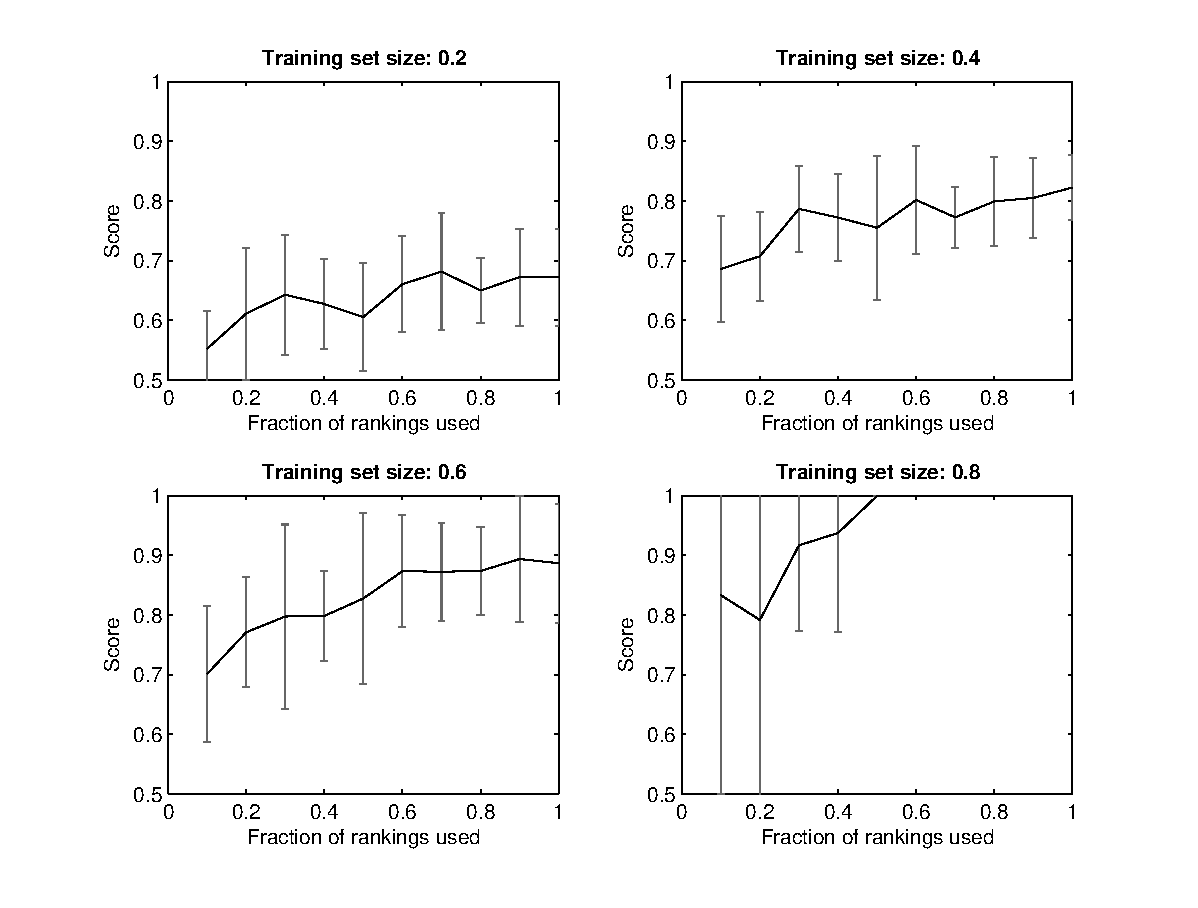
\includegraphics[width=1.1\linewidth]{rankings}
  \caption{Influence fraction of inequalities}
  \label{fig:fractie}
\end{figure}

Figure~\ref{fig:fractie} shows how the scores improve as the amount of examples and the fraction of included preferences increases.
In all cases, more than half the pairs of examples are correctly predicted and high scores can be obtained even for small datasets.
Additional experiments have shown that even for lower scores the learned optimization criteria are often capable of identifying the correct optimal solution.

The standard underlying model can be directly expressed using the soft constraints that can be learned.
Even though clausal theories can be very expressive, important restrictions have been placed on the learned clauses in this paper.
In order to test the accuracy for models which cannot be directly expressed, a model consisting of two disconnected clauses has been tested as well.
While there are limits to the expressibility, the learned optimization criteria were able to obtain similar scores and seem to be robust with respect to the exact formulation.

\begin{question}[Noise]
  What is the influence of noise on the accuracy?
\end{question}

The influence of noise is shown in figure~\ref{fig:ruis}.
Hereby, the second approach of testing is applied, using potentially overlapping train- and test sets.
High scores are obtained, even despite significant levels of noise.
The figure also shows that providing more rankings improves the robustness of the algorithm, even if the relative amount of noise remains unchanged.

\begin{figure}
  \centering
    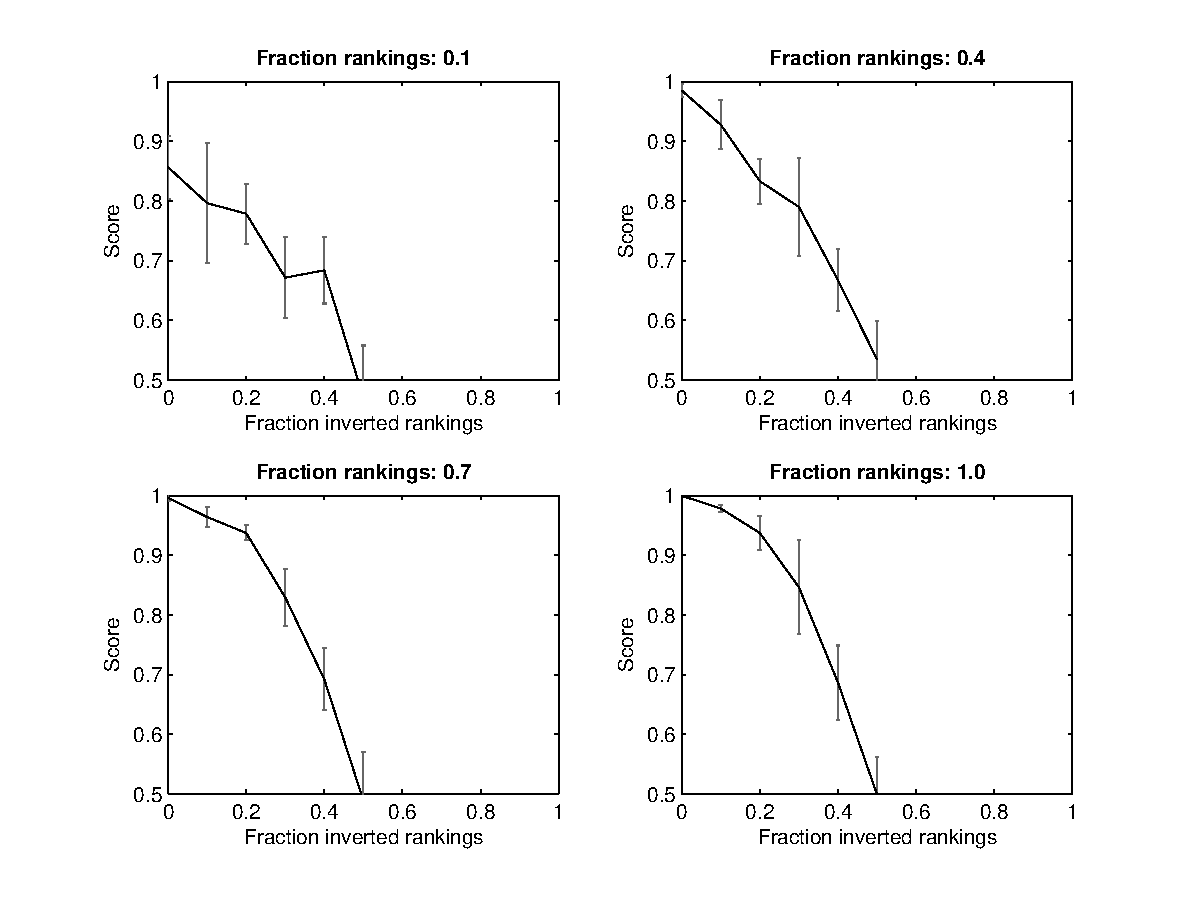
\includegraphics[width=1.1\linewidth]{noise}
  \caption{Influence of noise}
  \label{fig:ruis}
\end{figure}

\begin{question}[Threshold]
  What is the effect of the soft constraint threshold on the accuracy?
\end{question}
  \begin{table}
    \caption{Scores for different thresholds ($t$)}
    \begin{tabularx}{\linewidth}{XXXX}
      $t = 1$ & $t = 2$ & $t = 3$ & $t = 4$ \\
      \toprule
     0.823 & 0.740 & 0.788 & 0.735 \\
     ($\pm$ 0.073)&
($\pm$ 0.078)&
($\pm$ 0.074)&
($\pm$ 0.063)
    \end{tabularx}
    \label{tbl:limiet}
  \end{table}

Table~\ref{tbl:limiet} demonstrates that increasing the threshold used for finding soft constraints does not improve the score.
This experiment used 40\% of the examples as training set and 40\% of the available rankings.
However, if the size of the problem and examples is increased, a higher threshold will likely be appropriate.

% -------------------------------------------------
% Conclusion
% -------------------------------------------------

\section{Conclusion}
The research in this thesis has focused on automatically acquiring constraints and optimization criteria from examples and rankings.
Implementation for both clause learning and clausal optimization have been provided that accomplish these tasks using first order logic clauses.

The constraint learning implementation has been able to learn the relevant hard and soft constraints in all experiments.
For each problem, only a small number of examples was given to learn from.
The system requires only a minimal amount of information from the user, however, it also allows for the use of expressive background knowledge.
The learned constraints are domain independent, which facilitates the construction of positive examples.

Using the constraint learning implementation, the goal of learning optimization criteria has been accomplished.
Optimization criteria can be learned that enable optimal solutions to be found.
Even for small datasets and noisy rankings, constraints are found that enable most examples to be ranked correctly.

Aside from learning formal representations automatically from examples, this research shows how these representations can be used in practice.
This also forms an important step to enable the learning of optimization criteria in an interactive setting.

\paragraph{Future work}
This research offers multiple opportunities for future work.
It would be interesting to adapt the number of variables and literals in a clause dynamically.
This could be accomplished, for example, by using negative examples.
Learned clauses must be specific enough to not cover any negative examples. 

Additionally, it would be interesting to add interactivity to the learning system for the generation of examples or rankings.
Rankings expressing that examples are equally ranked are currently ignored.
Whenever provided explicitly, however, it could be interesting to incorporate this information into the algorithm.

As mentioned earlier, the domain independence of the clauses has several advantages.
In some cases, however, specific objects are inherently present in any problem instantiation.
The constraint learning system could be enhanced to include such global constants.

Finally, it would desirable to improve the implementation in order to tackle larger sized problems.
All the experiments were conducted with problems of limited size and the computation time increases rapidly if there are more predicates, variables and literals to be used in clauses.

\section*{Acknowledgments}
The author thanks his promoters Dr. Luc De Raedt en Dr. ir. Anton Dries.
Furthermore, he expresses his gratitude for the help provided by Bart Bogaerts, Dr. Jesse Davis, Dr. Marc Denecker and Vladimir Dzyuba.

\newpage

%
% ---- Bibliography ----
%
\bibliographystyle{aaai}
\bibliography{Bibliography}
\end{document}
